\begin{figure}[htbp] \centering
\subsection{BDD Hardware}
{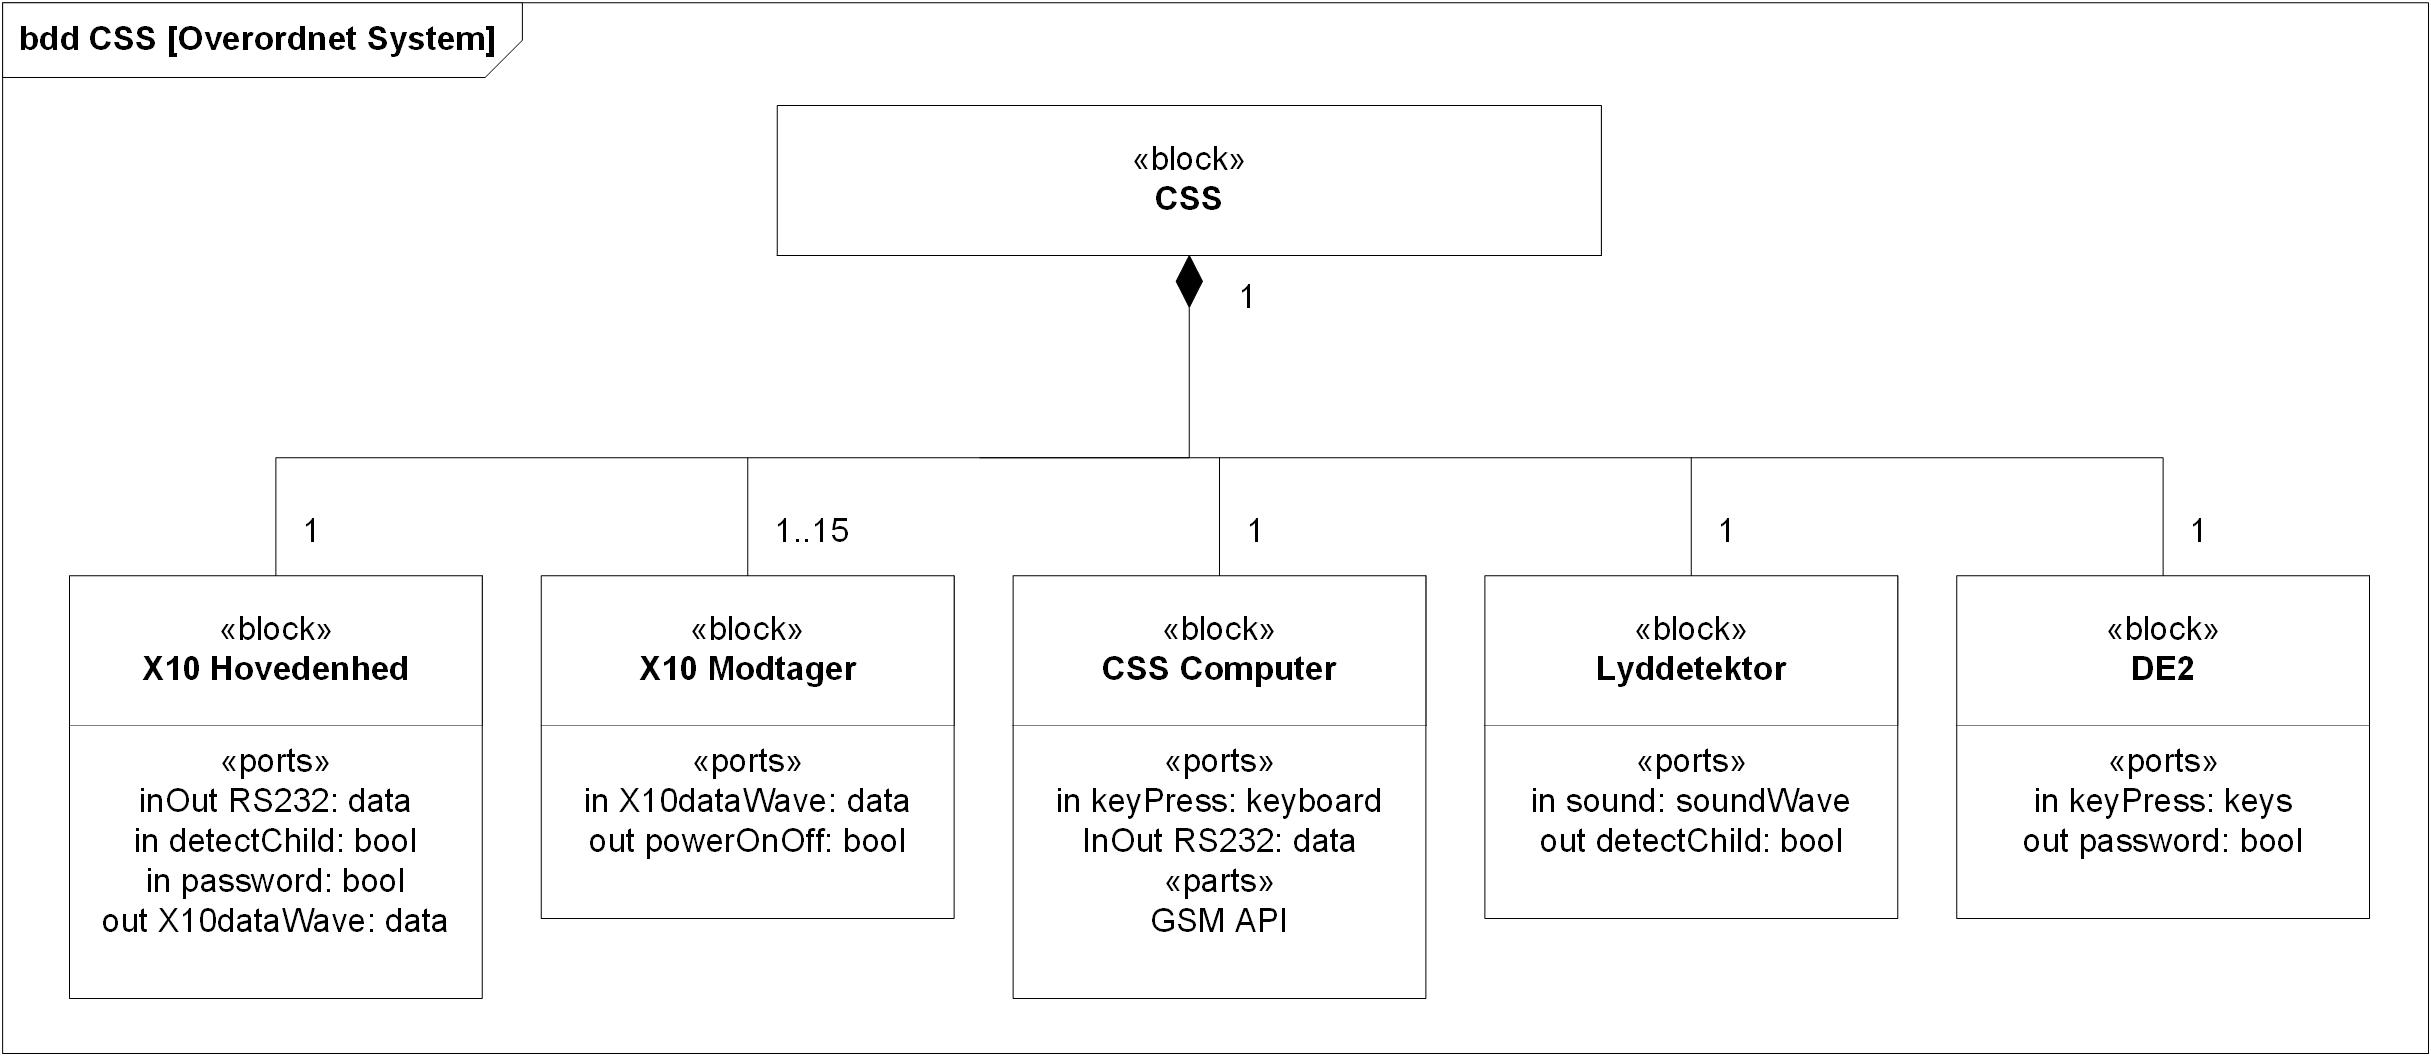
\includegraphics[width=0.9\textwidth]{billeder/diagrammer/BDD_Hardware}}
\caption{BDD Hardware}
\label{lab:bddhardware}
\end{figure}
BDD diagrammet giver et overblik over hvad det samlede system består af. Vi ser en port beskrivelse som viser hvilke signaler hver blok består af.

\begin{figure}[htbp] \centering
\subsection{BDD Hovedenhed}
{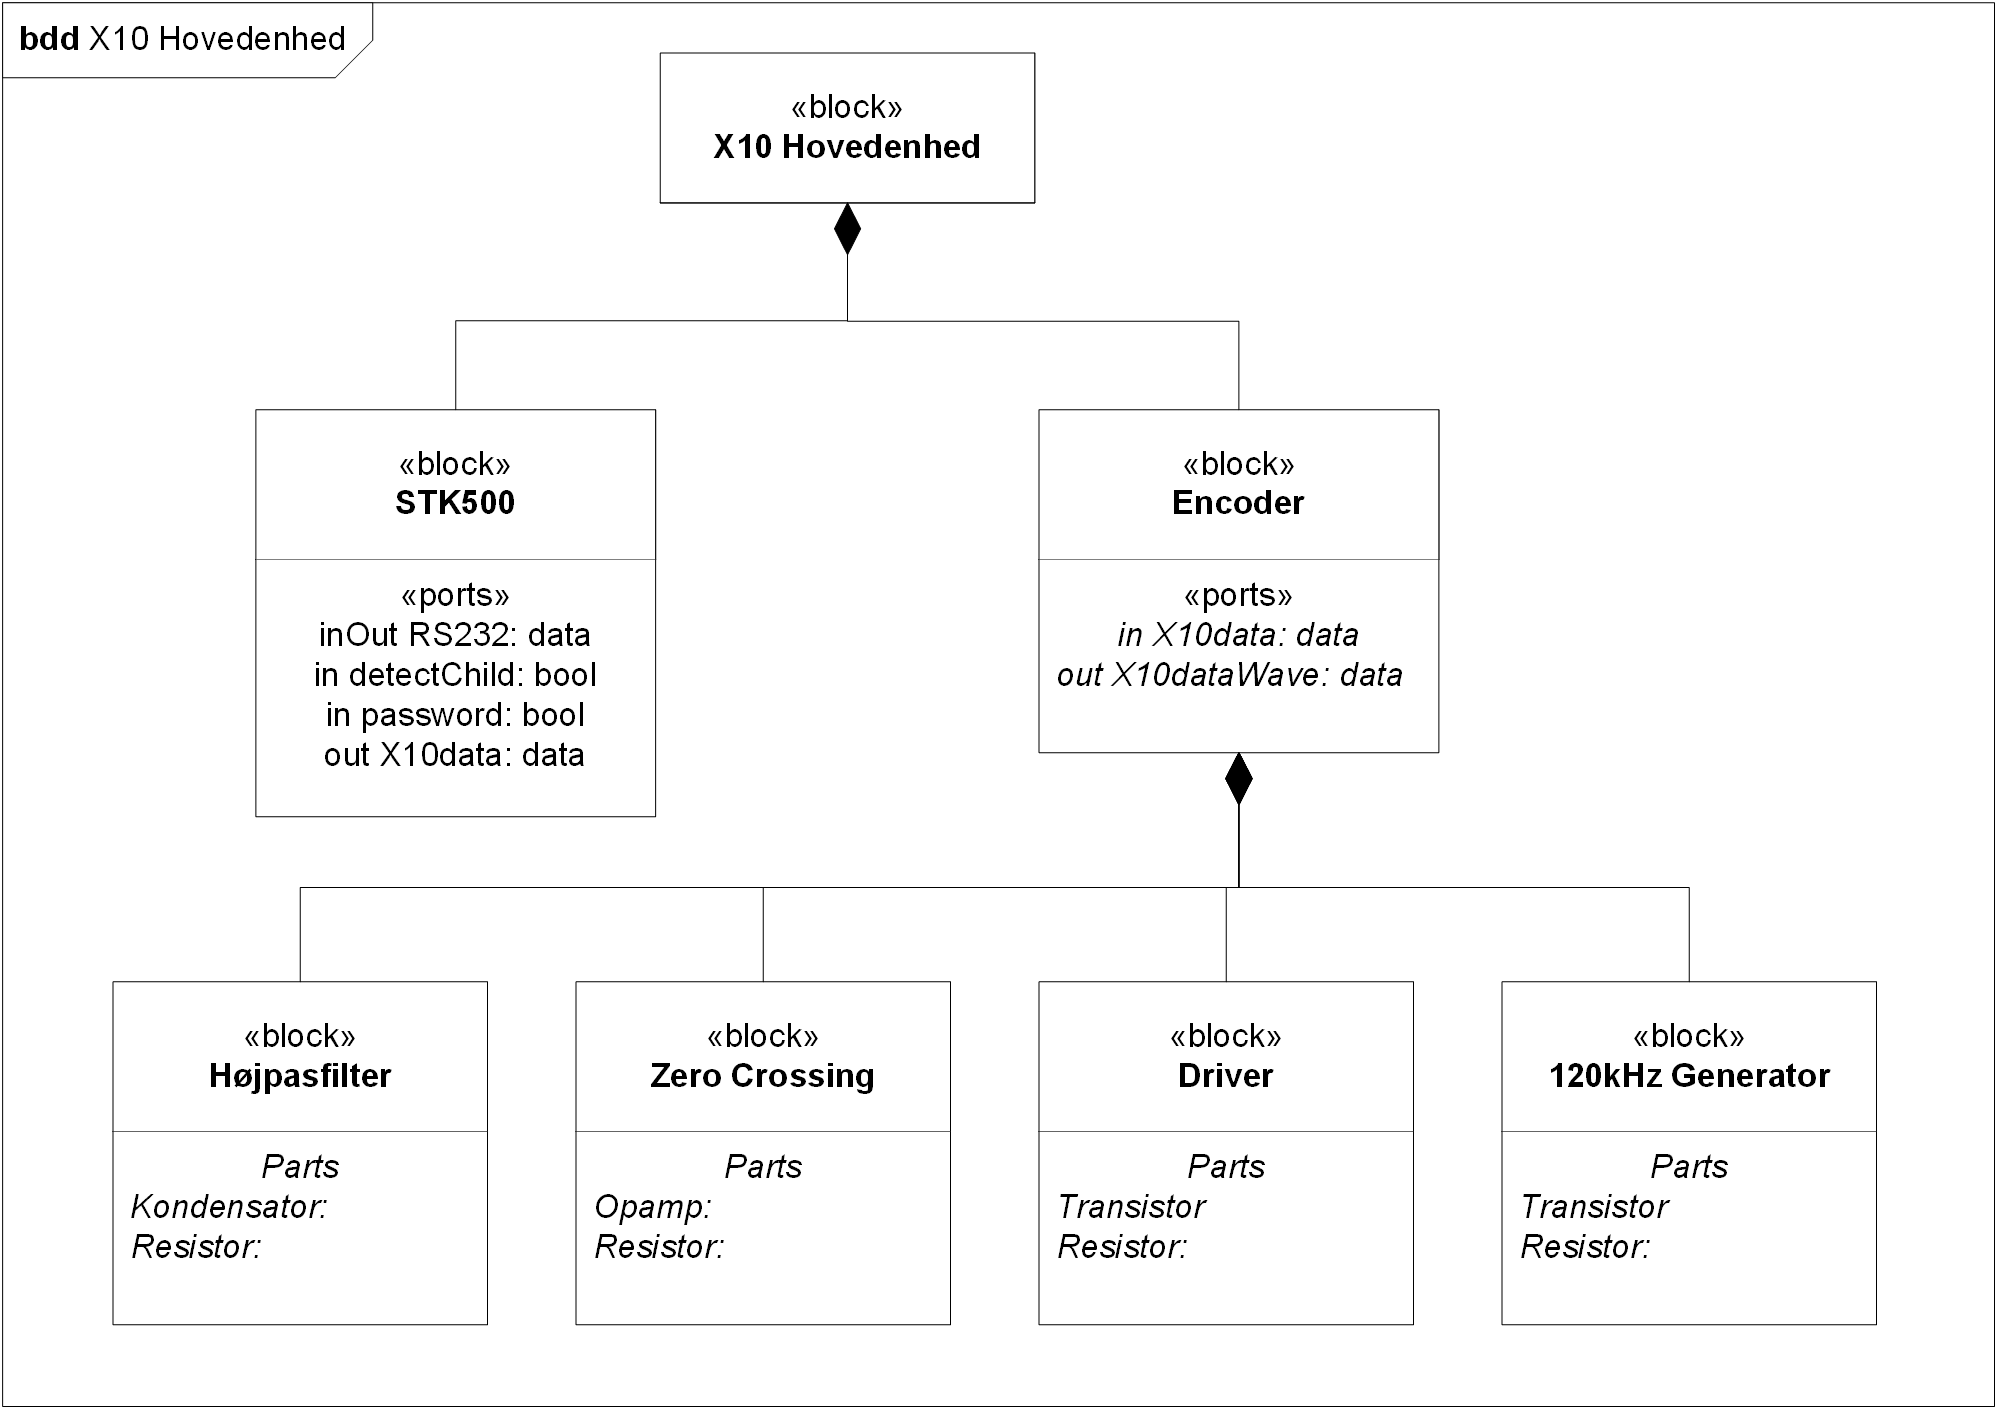
\includegraphics[width=0.9\textwidth]{billeder/diagrammer/BDD_Hovedenhed}}
\caption{BDD Hovedenhed}
\label{lab:bddhovedenhed}
\end{figure}
BDD diagrammet giver et overblik over hvad CSS hovedenheden består af. Vi ser en portbeskrivelse for STK kittet og encoder samt et overblik over hvilke komponenter encoderen består af. 

\begin{figure}[htbp] \centering
\subsection{BDD Modtager}
{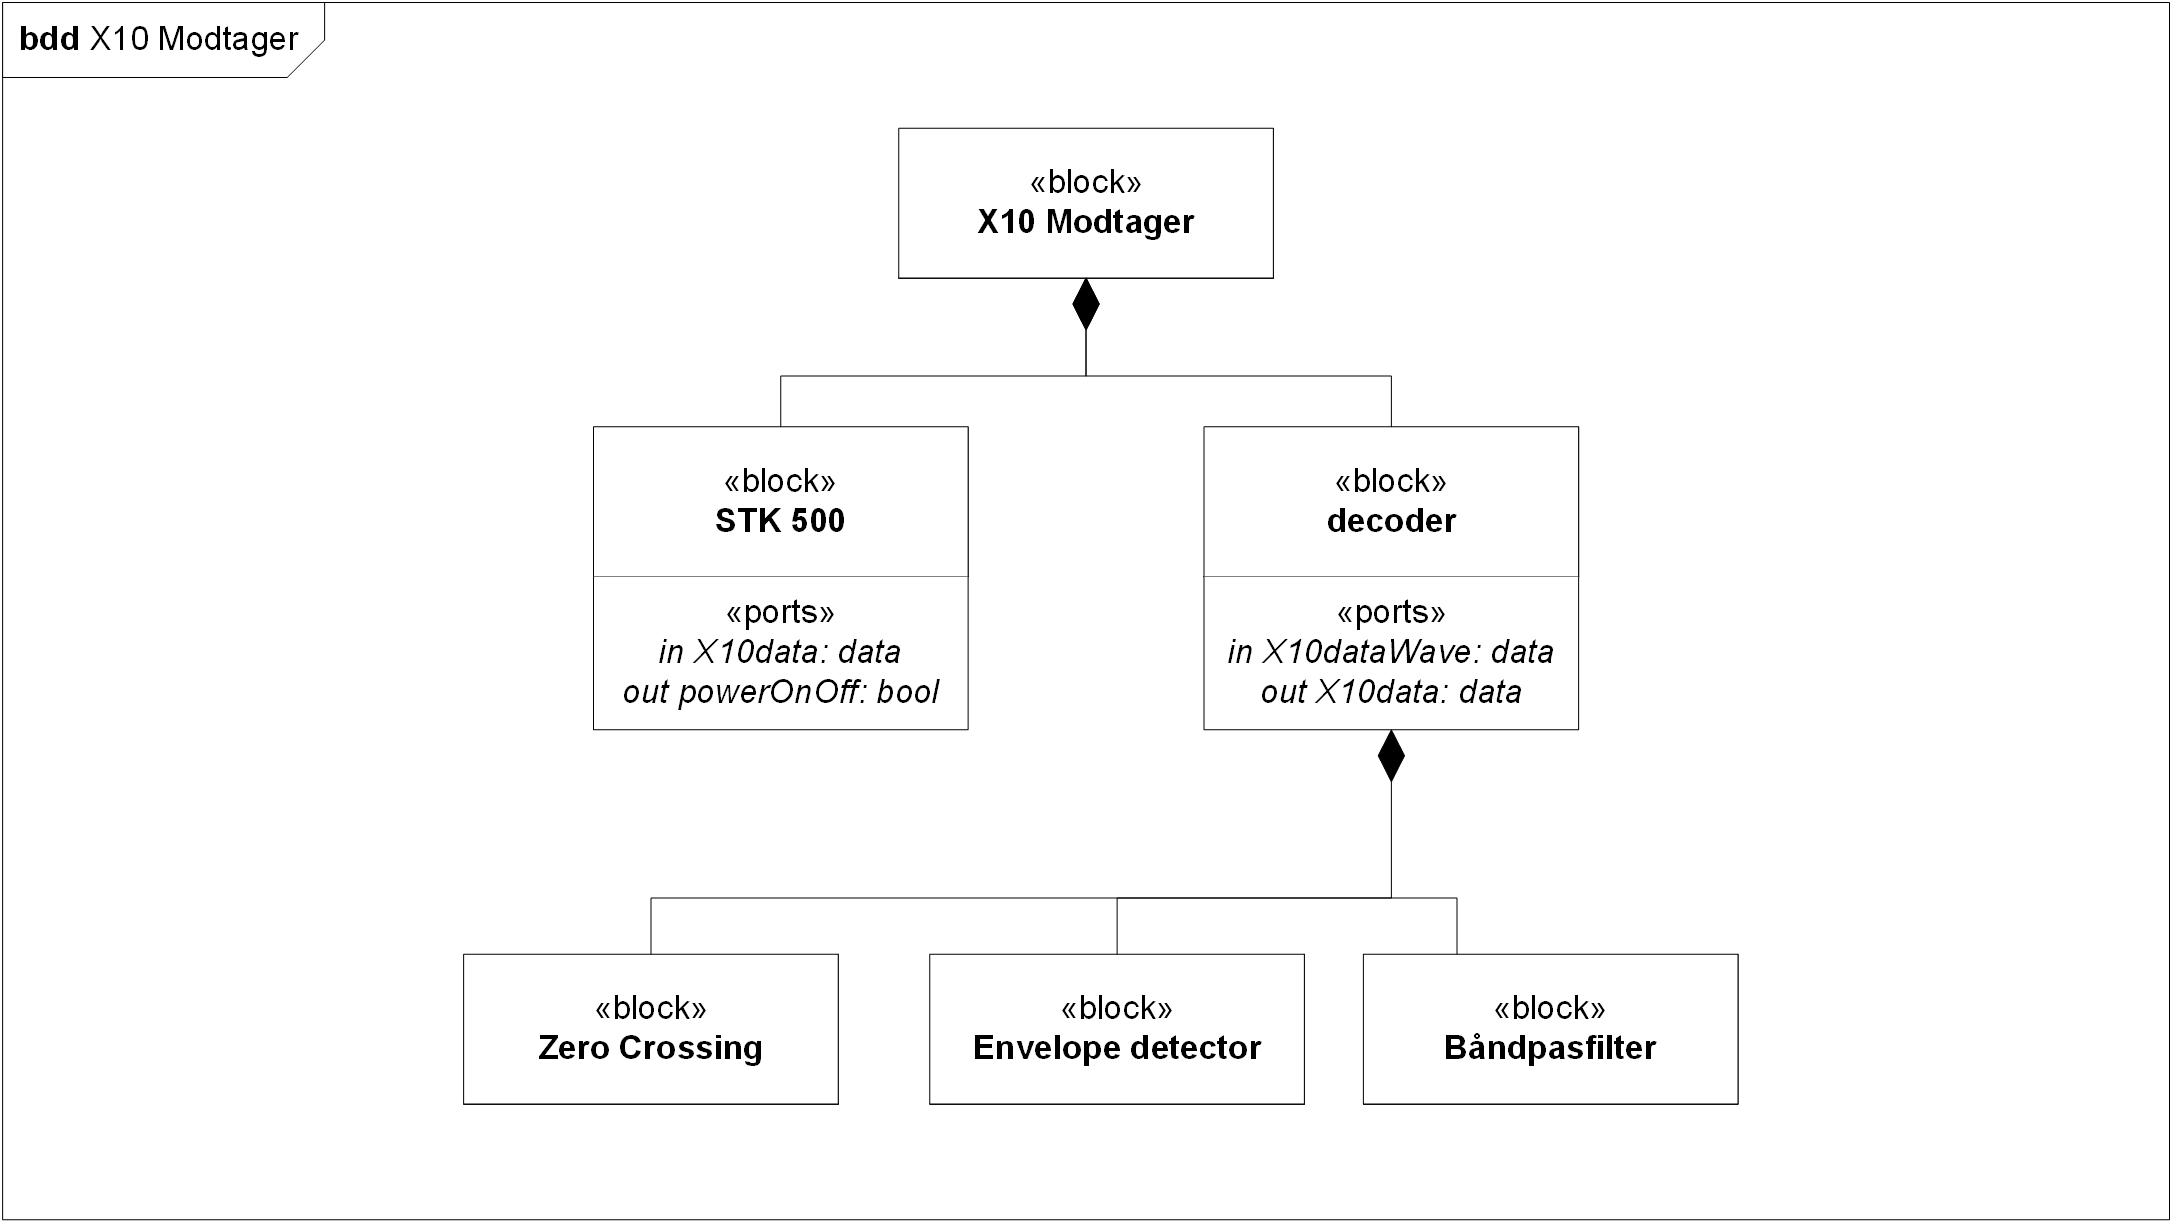
\includegraphics[width=0.9\textwidth]{billeder/diagrammer/BDD_Modtager}}
\caption{BDD Modtager}
\label{lab:bddmodtager}
\end{figure}
BDD diagrammet giver et overblik over hvad X10 modtageren består af. Vi ser en portbeskrivelse for STK kittet og decoderen samt et overblik over hvilke komponenter decoderen består af.

\begin{figure}[htbp] \centering
\subsection{IBD Hardware}
{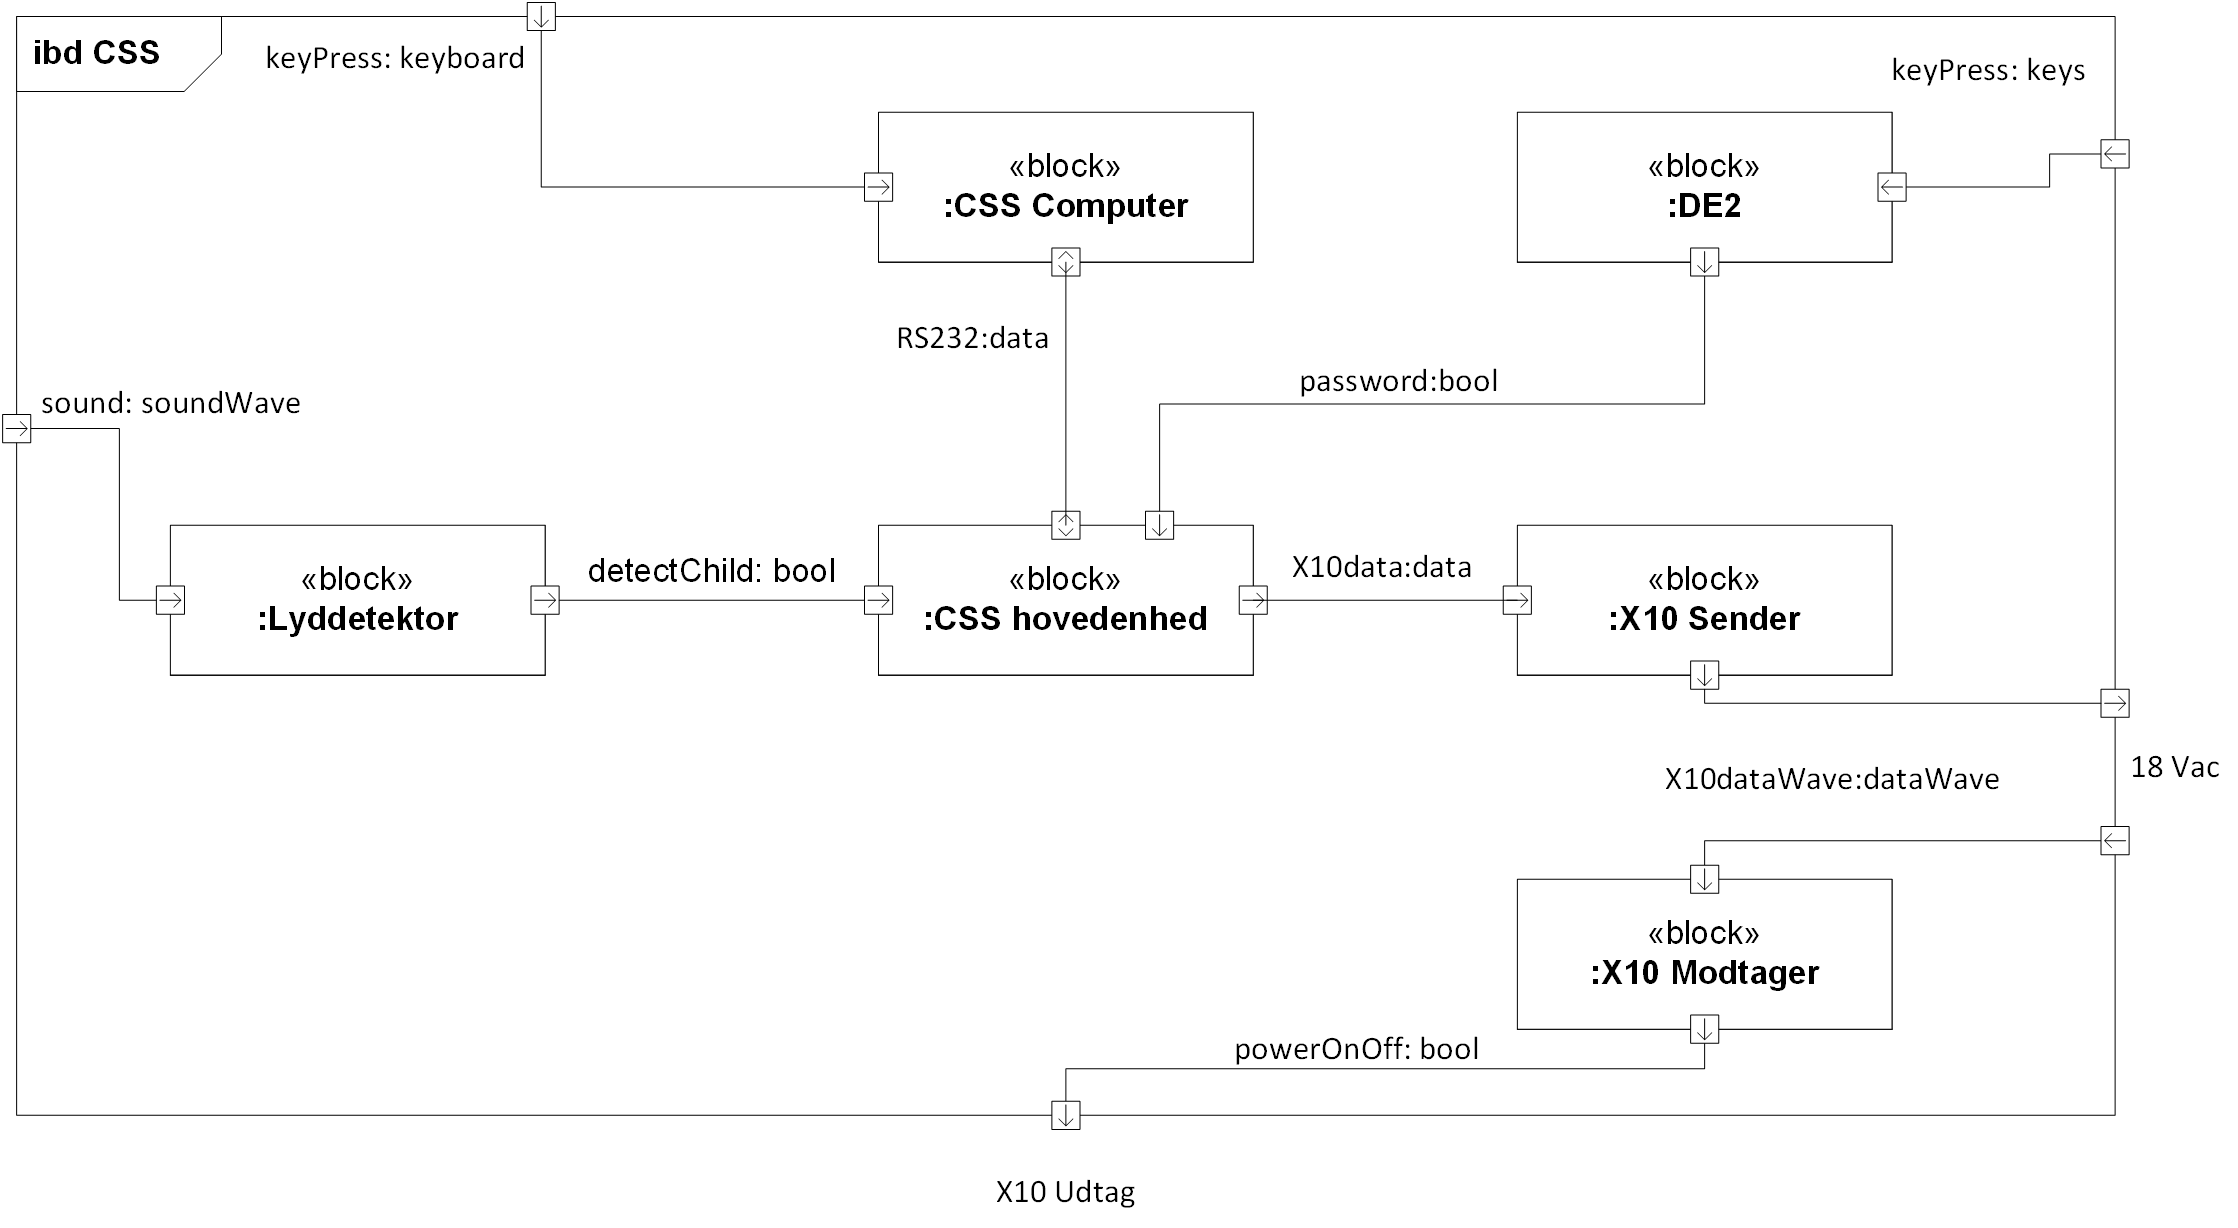
\includegraphics[width=0.9\textwidth]{billeder/diagrammer/IBD_Hardware}}
\caption{IBD Hardware}
\label{lab:ibdhardware}
\end{figure}
IBD diagrammet giver et internt overblik over hvordan hele vores system er forbundet. Vi ser hvilke type signaler der bliver sendt imellem vores forskellige blokke.

\begin{figure}[htbp] \centering
\subsection{IBD Hovedenhed og Modtager}
{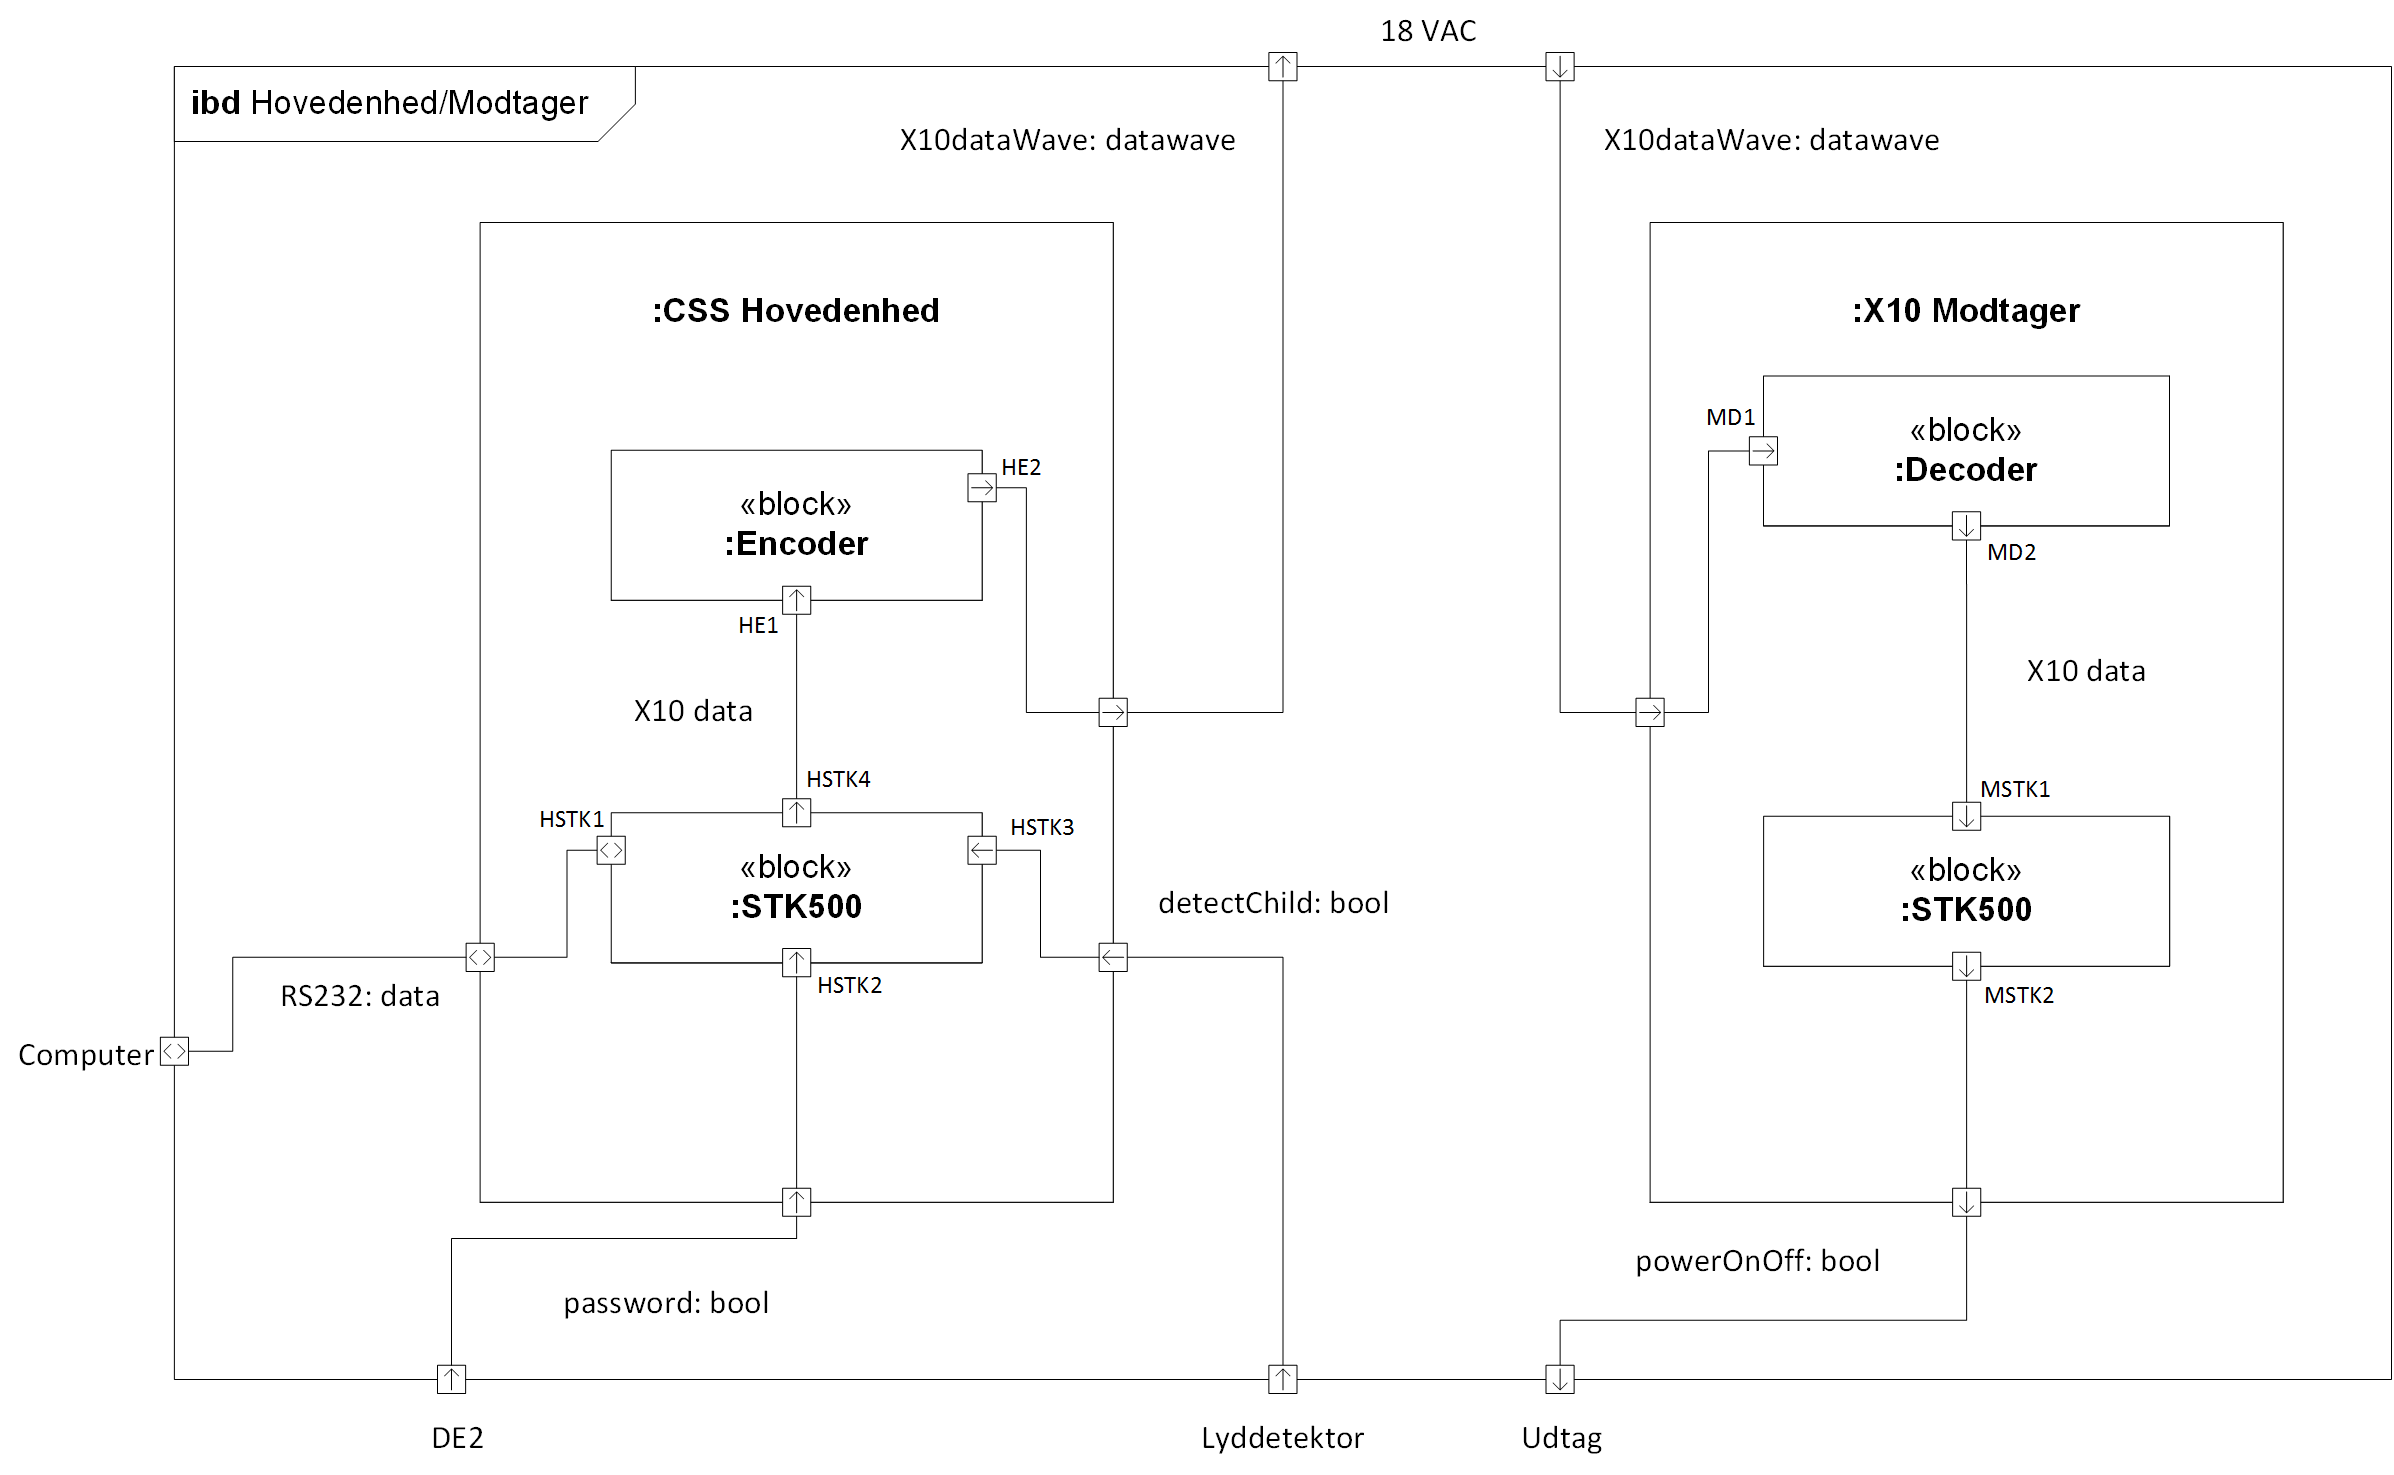
\includegraphics[width=0.9\textwidth]{billeder/diagrammer/IBD_Hovedenhed_Modtager}}
\caption{IBD Hovedenhed og Modtager}
\label{lab:ibdhovedenhedmodtager}
\end{figure}
IBD diagrammet giver et internt overblik over hvordan vores X10 hovedenhed og X10 modtager er forbundet. Vi ser hvilke type signaler der bliver sendt imellem vores forskellige blokke.

\subsection{Signaltabel}

\subsubsection{Hovedenhed}
\begin{tabular}{|p{3cm}|p{2,4cm}|p{2,4cm}|p{2,4cm}|p{2,4cm}|}
\hline 
\textbf{Funktion} &\textbf{Område} &\textbf{Signaltype} &\textbf{Terminal 1} &\textbf{Terminal 2} \\ 
\hline 
\multicolumn{5}{|l|}{\textbf{:Encoder}} \\ 
\hline 
X10 data &databit &data &HE1 &HSTK4\\ 
\hline 
Send kommando ud på 18 V nettet &18 VAC \newline 120KHz &?? &HE2 &18 VAC\\ 
\hline 
\multicolumn{5}{|l|}{\textbf{:STK500}} \\ 
\hline 
RS232 datainput &RS232 &?? &HSTK1 &Computer\\ 
\hline 
Password bool  &0-5 V TTL &bool &HSTK2 &DE2\\ 
\hline 
Høj ved lyddektektion &0-5 V TTL &bool &HSTK3 &Lyddektektor\\ 
\hline 
X10 data &databit &data &HSTK4 &HE1\\ 
\hline 
\end{tabular} 

\subsubsection{Modtager}
\begin{tabular}{|p{3cm}|p{2,4cm}|p{2,4cm}|p{2,4cm}|p{2,4cm}|}
\hline 
\textbf{Funktion} &\textbf{Område} &\textbf{Signaltype} &\textbf{Terminal 1} &\textbf{Terminal 2} \\ 
\hline 
\multicolumn{5}{|l|}{\textbf{:Decoder}} \\ 
\hline 
Modtager kommando fra 18 V nettet &18 VAC \newline 120KHz &?? &MD1 &18 VAC\\ 
\hline 
X10 data &databit &data &MD2 &MSTK1\\ 
\hline 
\multicolumn{5}{|l|}{\textbf{:STK500}} \\ 
\hline 
X10 data &databit &data &MSTK1 &MD2\\ 
\hline 
Kommando signal til udtag  &0-5 V TTL &bool &MSTK2 &Udtag\\ 
\hline 

\end{tabular} 
